\section{41 - MAT - AG 4.1, AN 1.1, FA 5.1  - Krippenstein/five fingers - Matura 2013/14 2. Nebentermin}

\begin{langesbeispiel} \item[0] %PUNKTE DES BEISPIELS
				Die Dachsteinseilbahn erschließt vom oberösterreichischen Ort Obertraun aus den nördlichen Teil des Dachsteinmassivs. Die Dachsteinseilbahn besteht aus drei Teilstrecken. Die erste Teilstrecke auf die Schönbergalm ist bereits seit 1951 in Betrieb. Die zweite Teilstrecke führt von der Schönbergalm zum Krippenstein. Von dort aus ist die Aussichtsplattform \textit{five fingers} durch einen Fußweg erreichbar. Die dritte Teilstrecke führt vom Krippenstein weiter zur Gjaidalm. 
				
				Bei den folgenden Aufgabenstellungen werden Orte als Punkte modelliert. 

\subsection{Aufgabenstellung:}
\begin{enumerate}
	\item Die Bergstation Krippenstein $K_1$ und die Schönbergalm $S$ sind durch eine Seilbahn verbunden. Der Verlauf des Tragseils wird, wie in der nebenstehenden Abbildung dargestellt, modelliert. Dabei werden $x$ und $y$ in Metern gemessen.
	
	
	\begin{center}
	\resizebox{0.5\linewidth}{!}{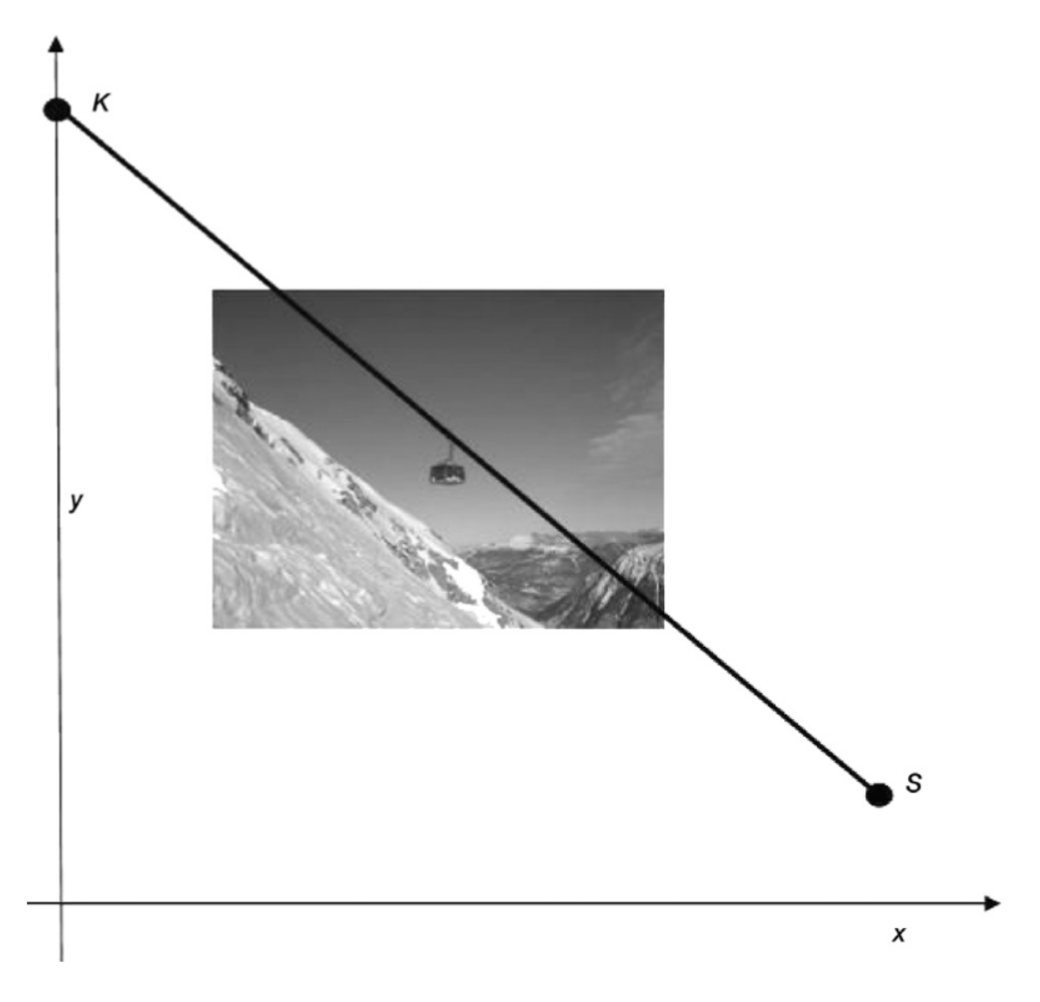
\includegraphics{../_database/Bilder/Bild41-1.eps}}
	\end{center}
	
	Nach dieser Modellierung gilt: $K=(0|2\,100)$ und $S=(2\,160|1\,350)$
	
	\fbox{A} Bestimme den Steigungswinkel des Tragseils!
	
	An welcher Stelle gleicher Seehöhe wie $S$ müsste die Talstation $S'$ stehen, wenn das Tragseil mit $100\,\%$ Steigung verlaufen soll?
	
	Gib die Koordinaten von $S'$ an!
	
		\item Mit zunehmender Höhe nimmt der Luftdruck exponentiell ab. Dabei gilt für die Höhe $h$ (gemessen in m über dem Meeresspiegel) und den Luftdruck $p$ (gemessen in mbar) näherungsweise der folgende funktionale Zusammenhang: $p(h)=1\,013,25\cdot e^{-0,000118\cdot h}$.
		
		Berechne die prozentuelle Druckabnahme auf der Fahrt von der Schönbergalm (Seehöhe $1\,350$\,m) bis zur Bergstation Krippenstein (Seehöhe 2\,100\,m)!
		
		Kreuze die zutreffende(n) Aussage(n) an!
		
		\multiplechoice[5]{  %Anzahl der Antwortmoeglichkeiten, Standard: 5
						L1={Die prozentuelle Druckabnahme pro Höhenmeter ist konstant.},   %1. Antwortmoeglichkeit 
						L2={Bei einer Verdopplung der Höhe halbiert sich der Luftdruck.},   %2. Antwortmoeglichkeit
						L3={Die absolute Druckabnahme pro Höhenmeter ist konstant.},   %3. Antwortmoeglichkeit
						L4={Der zur Funktion $p$ gehörige Graph ist streng monoton fallend.},   %4. Antwortmoeglichkeit
						L5={Der zur Funktion $p$ gehörige Graph nähert sich asymptotisch der waagrechten Achse.},	 %5. Antwortmoeglichkeit
						L6={},	 %6. Antwortmoeglichkeit
						L7={},	 %7. Antwortmoeglichkeit
						L8={},	 %8. Antwortmoeglichkeit
						L9={},	 %9. Antwortmoeglichkeit
						%% LOESUNG: %%
						A1=1,  % 1. Antwort
						A2=4,	 % 2. Antwort
						A3=5,  % 3. Antwort
						A4=0,  % 4. Antwort
						A5=0,  % 5. Antwort
						}
						\end{enumerate}\leer
				
\antwort{
\begin{enumerate}
	\item \subsection{Lösungserwartung:} 
	
		$\tan(\alpha)=\frac{750}{2\,160}\Rightarrow\alpha\approx 19,15^\circ$ bzw. $\alpha\approx 0,3342$\,rad
		
		$S'=(750|1\,350)$
	 	
	\subsection{Lösungsschlüssel:}
	\begin{itemize}
		\item  Ein Ausgleichspunkt für die korrekte Berechnung.
		
		Lösungsintervall: $[19^\circ;19,2^\circ]$ bzw. $[0,33\,\text{rad};0,335\,\text{rad}]$
		\item Ein Punkt für die korrekte Berechnung.
	\end{itemize}
	
	\item \subsection{Lösungserwartung:}
			
		$\dfrac{p(1\,350)-p(2\,100)}{p(1\,350)}\approx 0,085=8,5\,\%$
		
	\subsection{Lösungsschlüssel:}
	
\begin{itemize}
	\item  Ein Punkt für eine korrekte Berechnung. Lösungsintervall $[0,084;0,085]$ bzw. $[8,4\,\%;8,5\,\%]$.
	
	Lösungen aus dem Intervall $[-0,085;-0,084]$ bzw. $[-8,5\,\%;-8,4\,\%]$ sind ebenso als richtig zu werten.
	\item  Multiple-Choice-Aufgabe: Ein Punkt ist genau dann zu geben, wenn ausschließlich alle laut Lösungserwartung richtigen Antwortmöglichkeiten angekreuzt sind.

\end{itemize}

\end{enumerate}}
		\end{langesbeispiel}